\documentclass[12pt,a4paper]{article}
\usepackage[UTF8]{ctex}
\usepackage{amsmath,amssymb}
\usepackage{xcolor}
\usepackage{hyperref}
\usepackage{geometry}
\usepackage{graphicx}
\geometry{margin=2.5cm}

\title{Basic Gates / 基本量子门}
\author{QuoNic}
\date{}

\begin{document}
\maketitle

\begin{center}
\textbf{Foundational / 基础} | 难度：初级 | 预计时间：10 分钟
\end{center}

\tableofcontents
\newpage

\section{为什么需要？}

基本量子门是量子计算的基础构建块。

\subsection{经典局限}
\begin{itemize}
  \item 经典逻辑门（AND、OR、NOT）是不可逆的
  \item 经典门无法创建叠加态
  \item 经典门无法创建纠缠态
\end{itemize}

\subsection{量子优势}
\begin{itemize}
  \item 量子门是可逆的
  \item 可以创建叠加态和纠缠态
  \item 是量子计算的基础
\end{itemize}

\subsection{实际应用}
\begin{itemize}
  \item 量子计算
  \item 量子通信
  \item 量子密码学
\end{itemize}

\section{快速上手}

\begin{verbatim}
from quonic import qgate, qshow
from quonic.gates import X, H, Z

qgate(X, 0)  # Pauli-X (NOT gate)
qgate(H, 0)  # Hadamard
qgate(Z, 0)  # Pauli-Z (phase flip)
qshow()
\end{verbatim}

\textbf{预期输出}：
\begin{verbatim}
backend: native | shots: 1024
Result:
  |0>     512  ( 50.0%)  ####################
  |1>     512  ( 50.0%)  ####################
\end{verbatim}

\section{原理详解}

\subsection{电路图}

\begin{center}
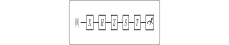
\includegraphics[width=0.6\textwidth]{../../images/basic_gates_circuit.svg}
\end{center}

\subsection{数学推导}

\textbf{Pauli-X 门}（NOT 门）：
\begin{equation}
X = \begin{pmatrix} 0 & 1 \\ 1 & 0 \end{pmatrix}
\end{equation}
\begin{equation}
X|0\rangle = |1\rangle, \quad X|1\rangle = |0\rangle
\end{equation}

\textbf{Hadamard 门}：
\begin{equation}
H = \frac{1}{\sqrt{2}} \begin{pmatrix} 1 & 1 \\ 1 & -1 \end{pmatrix}
\end{equation}
\begin{equation}
H|0\rangle = \frac{|0\rangle + |1\rangle}{\sqrt{2}}, \quad H|1\rangle = \frac{|0\rangle - |1\rangle}{\sqrt{2}}
\end{equation}

\textbf{Pauli-Z 门}（相位翻转）：
\begin{equation}
Z = \begin{pmatrix} 1 & 0 \\ 0 & -1 \end{pmatrix}
\end{equation}
\begin{equation}
Z|0\rangle = |0\rangle, \quad Z|1\rangle = -|1\rangle
\end{equation}

\textbf{Pauli-Y 门}：
\begin{equation}
Y = \begin{pmatrix} 0 & -i \\ i & 0 \end{pmatrix}
\end{equation}
\begin{equation}
Y|0\rangle = i|1\rangle, \quad Y|1\rangle = -i|0\rangle
\end{equation}

\textbf{S 门}（相位门）：
\begin{equation}
S = \begin{pmatrix} 1 & 0 \\ 0 & i \end{pmatrix}
\end{equation}
\begin{equation}
S|0\rangle = |0\rangle, \quad S|1\rangle = i|1\rangle
\end{equation}

\textbf{T 门}（$\pi/8$ 门）：
\begin{equation}
T = \begin{pmatrix} 1 & 0 \\ 0 & e^{i\pi/4} \end{pmatrix}
\end{equation}
\begin{equation}
T|0\rangle = |0\rangle, \quad T|1\rangle = e^{i\pi/4}|1\rangle
\end{equation}

\subsection{几何解释}

在 Bloch 球上：
\begin{itemize}
  \item X 门：绕 X 轴旋转 $\pi$
  \item Y 门：绕 Y 轴旋转 $\pi$
  \item Z 门：绕 Z 轴旋转 $\pi$
  \item H 门：绕 (X+Z)/$\sqrt{2}$ 轴旋转 $\pi$
  \item S 门：绕 Z 轴旋转 $\pi/2$
  \item T 门：绕 Z 轴旋转 $\pi/4$
\end{itemize}

\section{代码详解}

\begin{verbatim}
from quonic import qgate, qshow
from quonic.gates import X, H, Z, Y, S, T

# 单量子比特门
qgate(X, 0)  # Pauli-X: |0> -> |1>, |1> -> |0>
qgate(H, 0)  # Hadamard: |0> -> (|0>+|1>)/sqrt(2)
qgate(Z, 0)  # Pauli-Z: |0> -> |0>, |1> -> -|1>
qgate(Y, 0)  # Pauli-Y: |0> -> i|1>, |1> -> -i|0>
qgate(S, 0)  # S gate: |0> -> |0>, |1> -> i|1>
qgate(T, 0)  # T gate: |0> -> |0>, |1> -> e^(i*pi/4)|1>

qshow()
\end{verbatim}

\section{进阶用法}

\subsection{场景 1：受控门}

\begin{verbatim}
from quonic.gates import CX, CZ, CY

# CNOT gate
qgate(CX, 0, 1)  # Control: q0, Target: q1

# Controlled-Z gate
qgate(CZ, 0, 1)  # Control: q0, Target: q1

# Controlled-Y gate
qgate(CY, 0, 1)  # Control: q0, Target: q1
\end{verbatim}

\subsection{场景 2：旋转门}

\begin{verbatim}
from quonic.gates import Rx, Ry, Rz
import math

# Rx gate: rotation around X axis
qgate(Rx(math.pi/2), 0)  # Rotate pi/2 around X

# Ry gate: rotation around Y axis
qgate(Ry(math.pi/4), 0)  # Rotate pi/4 around Y

# Rz gate: rotation around Z axis
qgate(Rz(math.pi), 0)  # Rotate pi around Z
\end{verbatim}

\subsection{场景 3：多量子比特门}

\begin{verbatim}
from quonic.gates import CCX, CSWAP

# Toffoli gate (CCX)
qgate(CCX, 0, 1, 2)  # Control: q0, q1; Target: q2

# Fredkin gate (CSWAP)
qgate(CSWAP, 0, 1, 2)  # Control: q0; Swap: q1, q2
\end{verbatim}

\section{适用场景}

\subsection{量子计算}

基本量子门是所有量子算法的基础。

\subsection{量子通信}

量子门用于制备和操作量子态。

\subsection{量子密码学}

量子门用于量子密钥分发和量子加密。

\section{常见问题}

\subsection{量子门和经典门有什么区别？}

量子门是可逆的，经典门是不可逆的。量子门可以创建叠加态和纠缠态。

\subsection{哪些门是通用的？}

\{H, T, CNOT\} 构成通用量子门集。任何量子电路都可以用这些门近似。

\subsection{量子门的矩阵表示是什么？}

量子门用酉矩阵表示，满足 $U^\dagger U = I$。

\section{学习路径}

\subsection{前置知识}
\begin{itemize}
  \item 量子比特
  \item 量子测量
\end{itemize}

\subsection{继续学习}
\begin{itemize}
  \item 量子电路
  \item 量子算法
  \item 量子纠错
\end{itemize}

\section{完整示例代码}

\subsection{示例 1：基本量子门}

\begin{verbatim}
from quonic import qgate, qshow
from quonic.gates import X, H, Z

qgate(X, 0)
qgate(H, 0)
qgate(Z, 0)
qshow()
\end{verbatim}

\subsection{示例 2：受控门}

\begin{verbatim}
from quonic import qgate, qshow
from quonic.gates import CX, H

qgate(H, 0)
qgate(CX, 0, 1)
qshow()
\end{verbatim}

\section{下载}

\begin{itemize}
  \item [basic\_gates.py](https://github.com/ChrisLee0721/QuoNic/blob/main/examples/basic_gates/basic_gates.py)
\end{itemize}

\end{document}
